\chapter{}\label{sec:appendix_mydata}

\begin{figure}[h]
  \begin{subfigure}[b]{0.40\textwidth}
    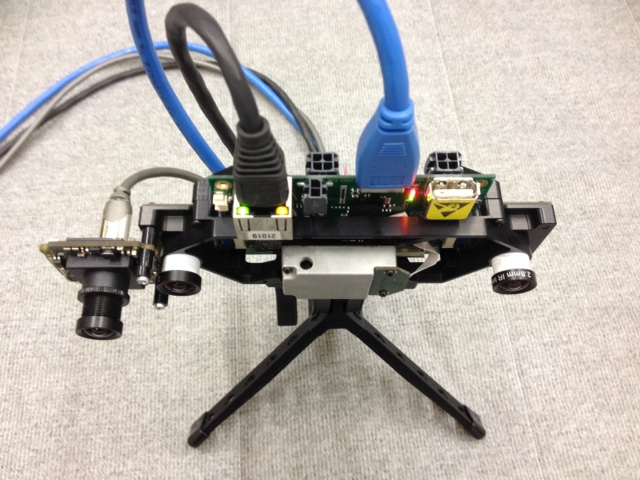
\includegraphics[width=\textwidth]{images/vi_bluefox.JPG}
    \caption{}
  \end{subfigure}
  \hfill
  \begin{subfigure}[b]{0.42\textwidth}
    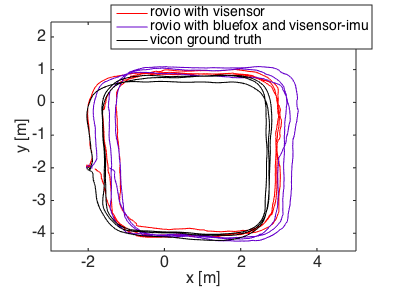
\includegraphics[width=\textwidth]{images/slow_2D.png}
    \caption{}
  \end{subfigure}
  \hfill
  \begin{subfigure}[b]{0.42\textwidth}
    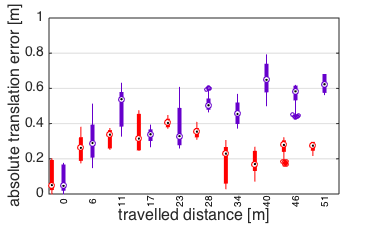
\includegraphics[width=\textwidth]{images/slow/slow_ate.png}
    \caption{}
  \end{subfigure}
  \begin{subfigure}[b]{0.42\textwidth}
    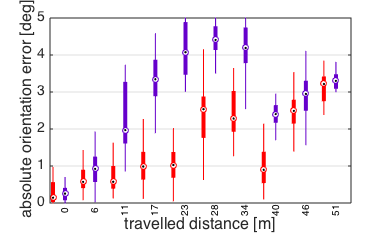
\includegraphics[width=\textwidth]{images/slow/slow_aoe.png}
    \caption{}
  \end{subfigure}
  \hfill
  \begin{subfigure}[b]{0.42\textwidth}
    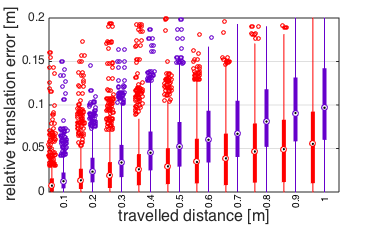
\includegraphics[width=\textwidth]{images/slow/slow_rte.png}
    \caption{}
  \end{subfigure}
  \hfill
  \begin{subfigure}[b]{0.42\textwidth}
    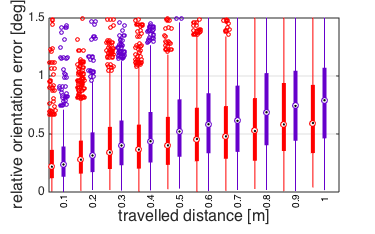
\includegraphics[width=\textwidth]{images/slow/slow_roe.png}
    \caption{}
  \end{subfigure}
   \caption{ROVIO results on the slow dataset with dynamics of $1.5\frac{m}{s}$ and $1\frac{rad}{s}$. (a) shows the sensor setup with bluefox camera and VI-sensor. (b) shows ROVIO's tracking performance for the hardware-wise time synchronized data (VI-sensor) and for the non time synchronized data (bluefox and VI-sensor-IMU). Regarding global accuracy (c and d) and local accuracy (e and f) ROVIO is performing better on the time synchronized than on the non time synchronized data. ROVIO is principally able to track the robot for both the time synchronized and the non time synchronized data.}
   \label{pics:appendix_slow}
\end{figure}

\begin{figure}[h]
  \begin{subfigure}[b]{0.40\textwidth}
    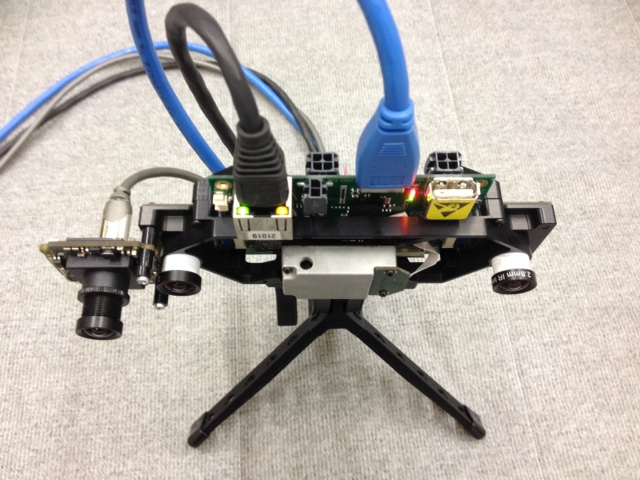
\includegraphics[width=\textwidth]{images/vi_bluefox.JPG}
    \caption{}
  \end{subfigure}
  \hfill
  \begin{subfigure}[b]{0.42\textwidth}
    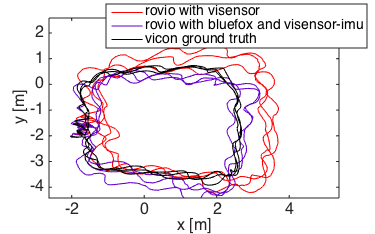
\includegraphics[width=\textwidth]{images/fast_fixed_2D.png}
    \caption{}
  \end{subfigure}
  \hfill
  \begin{subfigure}[b]{0.42\textwidth}
    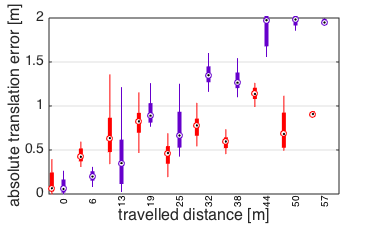
\includegraphics[width=\textwidth]{images/fast_fixed/fast_fixed_ate.png}
    \caption{}
  \end{subfigure}
  \begin{subfigure}[b]{0.42\textwidth}
    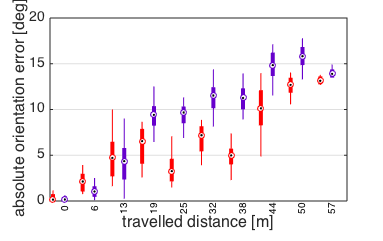
\includegraphics[width=\textwidth]{images/fast_fixed/fast_fixed_aoe.png}
    \caption{}
  \end{subfigure}
  \hfill
  \begin{subfigure}[b]{0.42\textwidth}
    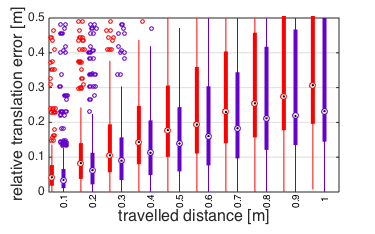
\includegraphics[width=\textwidth]{images/fast_fixed/fast_fixed_rte.png}
    \caption{}
  \end{subfigure}
  \hfill
  \begin{subfigure}[b]{0.42\textwidth}
    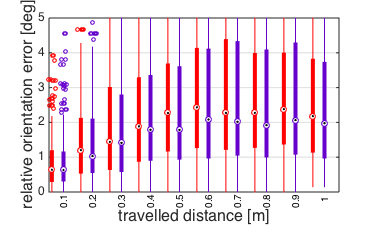
\includegraphics[width=\textwidth]{images/fast_fixed/fast_fixed_roe.png}
    \caption{}
  \end{subfigure}
   \caption{ROVIO results on the fast dataset with dynamics of $2.5\frac{m}{s}$ and $5\frac{rad}{s}$ and fixed extrinsics between camera and IMU. (a) shows the sensor setup with bluefox camera and VI-sensor. In section \ref{sec:timesync} it is demonstrated that ROVIO is diverging on this fast dataset when the extrinsics between camera and IMU are estimated online. By fixing the extrinsics on the hardware-wise non time synchronized setup, ROVIO is not diverging anymore. (b) shows the tracking performance of ROVIO for the time synchronized data (VI-sensor) and the non time synchronized data (bluefox and VI-sensor-IMU). The global accuracy (c and d) is better for the time synchronized data. The local accuracy (e and f) is surprisingly slightly better for the non time synchronized data, but very low for both setup. This dataset is lying at the dynamic limits of ROVIO and all errors are relatively high.}
   \label{pics:appendix_fast}
\end{figure}